\chapter{Golang}

\section{代理设置}
由于Golang是google的项目,因此,有的公用类库是依赖于google的域名解析的,导致在
一些情况下,无法更新或者下载相关的类库代码。解决方式就是设置代理。
Golang下载代码主要是通过go和其他一些版本控制工具进行下载的,通常的,版本控制工具
选择的都是git。因此,设置代理的时候,需要针对go和git设置。以windows为例。
\begin{code-block}{bash}
set http_proxy=http://10.1.1.10:8123
git config --global http.proxy http://10.1.1.10:8123
# 如果是使用sock5代理,则可以使用下面的方式
git config --global http.proxy socks5://localhost:8588
\end{code-block}

设置完成之后,即可进行go get更新和下载。Linux环境类似。

\section{安装Golang的开发工具}
只有设置好代理之后,才能正常的安装开发golang所需要使用的开发工具。
\begin{code-block}{bash}
go get -u -v honnef.co/go/tools/cmd/keyify
go get -u -v github.com/koron/iferr
go get -u -v github.com/visualfc/gocode
go get -u -v github.com/rogpeppe/godef
go get -u -v github.com/zmb3/gogetdoc
go get -u -v github.com/lukehoban/go-outline
go get -u -v github.com/sqs/goreturns
go get -u -v github.com/tpng/gopkgs
go get -u -v github.com/newhook/go-symbols
go get -u -v github.com/cweill/gotests/
go get -u -v github.com/alecthomas/gometalinter
go get -u -v github.com/jstemmer/gotags
go get -u -v github.com/klauspost/asmfmt/cmd/asmfmt
go get -u -v github.com/fatih/motion
go get -u -v github.com/fatih/gomodifytags
go get -u -v github.com/josharian/impl
go get -u -v github.com/kisielk/errcheck
go get -u -v github.com/sparrc/gdm
go get -u -v github.com/kardianos/govendor
go get -u -v github.com/tylerb/gotype-live
go get -u -v github.com/spf13/cobra/cobra
go get -u -v github.com/Masterminds/glide
go get -u -v github.com/golang/protobuf/protoc-gen-go
go get -v -u github.com/go-delve/delve/cmd/dlv
go get -u -v github.com/davidrjenni/reftools/cmd/fillstruct
go get -u -v github.com/golangci/golangci-lint/cmd/golangci-lint
go get -u -v github.com/bhcleek/lsp-position/cmd/lsp-position
go get -u -v github.com/golang/dep/cmd/dep
go get -u -v golang.org/x/lint/golint
go get -u -v golang.org/x/tools/gopls
go get -u -v golang.org/x/tools/cmd/guru
go get -u -v golang.org/x/tools/cmd/gorename
go get -u -v golang.org/x/tools/cmd/goimports
gometalinter --install -u
\end{code-block}

Golang代码补齐依赖于gocode,而gocode不是一个常驻的服务,也不是一个类似于
python或者c/c++一样的编译型的解释器。Gocode更类似于一个实时的代码分析服务器,
需要进行补齐时,访问gocode服务器,获取返回进行代码补齐。因此,最好是把gocode做成
一个常驻性的服务一直在后台运行,这需要对gocode的代码做部分的修改。
\begin{code-block}{bash}
cd go/src/github.com/nsf/gocode
git checkout -b backend
git revert e11212347fbcdc8a33e9955b141f250f4eb14e94
git commit
go build .
cp gocode.exe go/bin/
\end{code-block}

在windows下,后台程序一般是以服务的形式运行,所以,针对windows平台,我们可以通过
添加服务的方式添加gocode的常驻进程。
\begin{code-block}{bash}
sc create gocode binPath="c:\go\bin\gocode.exe set propose-builtins true autobuild true close-timeout 43200"
\end{code-block}
然后在windows服务中,启动gocode即可。

\begin{attention}
在windows当中,针对golang需要设置2个系统变量,一个是GOROOT,一个是GOPATH。在1.6
之前,GOROOT和GOPATH可以是同一个路径,但是,在1.8之后,GOROOT和GOPATH必须是不同的路径。
因此,如果执行go get命令,则下载的代码不会放到GOROOT当中,也就是说不能被go识别。
因此,如果一旦go get了第三方的代码,需要在自己的代码当中使用,则必须修改自己的GOPATH。
以windows为例,假设GOROOT=C:\textbackslash GO,GOPATH=C:\textbackslash GOLiberty,则自己的代码的GOPATH则需要修改为如下:
\begin{mdframed}[topline=false, bottomline=false, leftline=false, rightline=false, backgroundcolor=lbcolor]
\begin{minted}[fontsize=\scriptsize,linenos=false,breaklines=true]{bash}
set GOPATH=%GOPATH%;%cd%
\end{minted}
\end{mdframed}
\end{attention}

\section{模块初始化}
每个golang的模块都有一个隐藏的方法init,用来进行模块的初始化。当然,我们还可以进行
初始化的定制。具体就像下面一样
\begin{code-block}{go}
func init() {
    fmt.Printf("OS: %s, Arch: %s", runtime.GOOS, runtime.GOARCH)
}
\end{code-block}

\section{range的使用}
range通常用来进行迭代列表或者字典,通常的使用规则如下表\nameref{tab:usage_of_range}
\begin{center}
  \rowcolors{2}{green!80!yellow!50}{green!70!yellow!40}
  \begin{tabularx}{\textwidth}{|X|X|X|}
  \hline
  表达式类型& 第一返回值& 第二返回值\\ \hline
  [n]Ele& 数组索引值& 数组元素 \\
  string& 字符串索引& 字符数组对应的值\\
  map[k]v& map的键 & map键对应的值\\
  chan E & chan的元素 & - \\ \hline
  \end{tabularx}
  \label{tab:usage_of_range}
\end{center}

具体的使用如下
\begin{code-block}{go}
ints := []int{1, 2, 3, 4, 5, 6}
for index, value := range ints {
    fmt.Printf("%d: %d\n", index, value)
}
for index := range ints {
    fmt.Printf("%d: %d\n", index, ints[index])
}
dict := map[string]int{"lucifer": 18, "titans": 24, "garuda": 36}
for key, value := range dict {
    fmt.Printf("key is %s and value is %d\n", key, value)
}
\end{code-block}

\section{goto的使用}
goto的用法和c/c++当中的一样,也可以用来实现for循环,具体如下。
\begin{code-block}{go}
func goto_loop() {
    index := 0
loop:
    if index < 10 {
        fmt.Printf("index: \t%d\n", index)
        index++
        goto loop
    }
}
\end{code-block}

\section{闭包}
Golang支持闭包,但是和python的闭包不一样的是,golang的闭包可以对外层函数的变量
进行修改
\begin{code-block}{go}
func wrapper(start int) func(int) int {
    return func(input int) int {
        start = start + input
        return start
    }
}
\end{code-block}
上述代码在golang当中是合法的,但是,在python当中,是不能对外层函数的变量进行修改的
\begin{code-block}{python}
def wrapper(name):
    def _wrap(age):
        name = name + '.jpg'
        print('%s: %d\n' %(name, age))
    return _wrap


if __name__ == '__main__':
    w = wrapper('xx')
    w(12)
\end{code-block}
在python当中,上述代码就会出现错误:UnboundLocalError: local variable 'name' referenced before assignment

\section{Golang的继承}
Golang和c一样,并没有类的概念,因此没有继承。但是,由于golang有结构体的存在,因此,
可以使用组合的方式来实现继承。
\begin{code-block}{go}
type User struct{
    name string
    age uint
    address string
}

func (this *User) GetName() string{
    return this.name
}

type Student struct{
    User
    class string
    score uint
    order uint
}
\end{code-block}

在上边的例子中,Student结构内嵌了一个User结构,其结果就是Student结构也存在name,age
address等等属性,并且,GetName方法同样对Student结构是适用的。

\section{Golang的命令行参数}
和Python一样,golang提供了命令行处理的类库。比较常用的就是flag。
例子如下:
\begin{code-block}{go}
var (
    flag_name = flag.String("name", "demo", "The name of user. String value")
    flag_age  = flag.Int("age", 18, "The age of user. Int value")
)

func show_usage() {
    fmt.Fprintf(os.Stderr, "Usage: %s [-name] [-age]\n\n", os.Args[0])
    fmt.Fprintf(os.Stderr, "Flags:\n")
    flag.PrintDefaults()
}

func main(){
    flag.Usage = show_usage
    flag.Parse()
    fmt.Println(*flag_name)
    fmt.Println(*flag_age)
}
\end{code-block}

\section{Golang的Json处理}
同其他语言一样,golang也提供了json的处理,但是和python有不同。Python通常是将json和
字典(dict)进行相互转换,但是,golang只能是将struct对象转换为json,以及将json转换为
golang的映射(map,也即是python的字典)或者对象。另外,由于golang的struct的大小写规则,
如果struct的属性设置为小写,则无法被转换,这时候,需要用到大量的struct tag属性。
具体如下的例子。
\begin{code-block}{go}
import(
    "encoding/json"
)
type User struct {
    Id     string `json:"id"`
    Name   string `json:"name"`
    Active bool   `json:"active"`
    // omitempty表示该项如果有值就输出,否则隐藏
    // about表示该键在转换为json时,Bio键被转换为about键
    Bio       string `json:"about,omitempty"`
    Admin     bool   `json:"-"`  // -表示不输出该值
    AdminRole bool   `json:"-,"` // -,表示该键输出为-
}

func ConstomJson() {
    user := &User{Id: uuid.NewV4().String(), Name: "zhangjl",
                  Active: true, Bio: "luoyan", Admin: true, AdminRole: false}
    user_json, _ := json.Marshal(user)
    fmt.Printf("%v\n", string(user_json))

    user = &User{Id: uuid.NewV4().String(), Name: "zhangjl",
                 Active: true, Admin: true, AdminRole: true}
    // 将对象格式化为json数据
    user_json, _ = json.Marshal(user)
    fmt.Printf("%v\n", string(user_json))
    fmt.Printf("%s\n", user_json)
    // json.Marshal转换的结果是byte数组,将其转换为string
    fmt.Printf("%s\n", bytes.NewBuffer(user_json).String())

    json_str := `{"id":"7722a662-ceeb-41d4-9de7-f7132da3f985",
                  "name":"zhangjl","active":true,"-":false}`

    var f interface{}
    // 将json格式的字符串转换
    err := json.Unmarshal([]byte(json_str), &f)
    if err != nil {
        return
    }
    fmt.Printf("%v\n", f)

    // 转换为map结构
    m := f.(map[string]interface{})
    fmt.Printf("%v\n", m)
    fmt.Printf("%t\n", m["active"])
    fmt.Printf("%t\n", m["-"])

    var user_ User
    // 转换为golang定义的对象
    err = json.Unmarshal([]byte(json_str), &user_)
    if err != nil {
        return
    }
    fmt.Printf("%v\n", user_)
}
\end{code-block}

\section{Golang交叉编译}
Go是一门编译型语言,所以在不同平台上,需要编译生成不同格式的二进制包。
编译时候只需要指定两个参数:GOOS和GOARCH即可。
\begin{code-block}{bash}
# 编译到 linux 64bit
GOOS=linux GOARCH=amd64 go build
# 或者可以使用 -o 选项指定生成二进制文件名字
GOOS=linux GOARCH=amd64 go build -o app.linux

# 编译到 linux 32bit
GOOS=linux GOARCH=386 go build

# 编译到 windows 64bit
GOOS=windows GOARCH=amd64 go build

# 编译到 windows 32bit
GOOS=windows GOARCH=386 go build
\end{code-block}

如果是在windows上进行交叉编译,则操作有部分差别。
\begin{code-block}{bash}
set GOOS=linux
set GOARCH=amd64
go build
\end{code-block}

如果是需要CGO支持的,则需要使用交叉编译的C Complier。以在X86上交叉编译ARM的为例:
\begin{code-block}{bash}
wget https://releases.linaro.org/archive/15.06/components/toolchain/binaries/4.8/arm-linux-gnueabihf/\
gcc-linaro-4.8-2015.06-x86_64_arm-linux-gnueabihf.tar.xz

tar -Jxf gcc-linaro-4.8-2015.06-x86_64_arm-linux-gnueabihf.tar.xz
export CROSS_COMPILE=/opt/gcc-linaro-4.8-2015.06-x86_64_arm-linux-gnueabihf/bin/arm-linux-gnueabihf-

GOOS=linux GOARCH=arm CGO_ENABLED=1 \
    CC_FOR_TARGET=/opt/gcc-linaro-4.8-2015.06-x86_64_arm-linux-gnueabihf/bin/arm-linux-gnueabihf-gcc \
    CC=/opt/gcc-linaro-4.8-2015.06-x86_64_arm-linux-gnueabihf/bin/arm-linux-gnueabihf-gcc \
    go install

\end{code-block}

\section{Golang的坑爹问题}
Go毕竟还只是发展阶段的语言,存在一些问题是有可能的。下面记录一些实际当中遇到的
golang的坑.
\begin{outline}[enumerate]

  \1 ioutil ReadAll导致程序hang住

  Ioutil的ReadAll方法,在某些情况下,会导致程序被卡住,多见于在http请求时候,读取
  返回的body。一般发生在windows环境上,linux环境较少出现。解决的方法比较另类:设置
  http的keepalive参数为false即可。
\begin{code-in-enumerate}{go}
transport := &http.Transport{DisableKeepAlives: true}
client := &http.Client{Transport: transport}
\end{code-in-enumerate}

  \1 中文的使用

  Golang当中,中文字符占用3个字节
\begin{code-in-enumerate}{go}
fmt.Printf("%d\n", len("hello 北京")) // 得到的结果是12
\end{code-in-enumerate}

  对包含中文字符的字符串进行遍历时,需要转换为rune类型的切片,否则会出现乱码
\begin{code-in-enumerate}{go}
zh := "hello 北京"
for i := 0; i < len(zh); i++ {
    fmt.Printf("%c ", zh[i]) // 中文输出为乱码
}

rune_ := []rune(zh)
for i := 0; i < len(rune_); i++ {
    fmt.Printf("%c ", rune_[i]) // 正常输出为中文
}
\end{code-in-enumerate}

  \1 string与byte的相互转换

  Golang当中,byte实际上就是数字,可以使用\%d输出数值,也可以使用\%c输出为字符类型,
  从底层说,golang当中的string实质就是byte数组,因此二者可以相互转换。比如byte数组
  转换为string
\begin{code-in-enumerate}{go}
b := []byte{'a', 'b', 'c', 'd'}
str := string(b)
\end{code-in-enumerate}

  Golang的string转换为byte
\begin{code-in-enumerate}{go}
_b := []byte(str)
\end{code-in-enumerate}

  \1 timer,ticker与time.After的使用

\begin{code-in-enumerate}{go}
ticker := time.NewTicker(time.Second * 1)
timer := time.NewTimer(time.Second * 10)
timeout_5 := time.After(time.Second * 5)

for_select:
for {
    select {
        case <-ticker.C:
            fmt.Printf("Now is %s\n", time.Now().Format(
                "2006-01-02 15:04:05.000000"))
        case <-timeout_5:
            fmt.Printf("After 5 seconds\n")
        case <-timer.C:
            fmt.Printf("Time is up, break out the for-select\n")
            ticker.Stop()
            timer.Stop()
            break for_select
    }
}
\end{code-in-enumerate}

  \1 数组和切片的区别

  Golang当中,数组是数值类型,切片是引用类型。数组和切片的定义类似,但是数组在定义时
  需要指明长度,而切片定义则无需,如下
\begin{code-in-enumerate}{go}
arrays_int := [5]int{1,2,3,4,5} // arrays
arrays_int_copy := [...]int{1,2,3,4,5} //arrays, 自动推导模式
slice_int := []int{1,2,3,4,5} // slice
slice_copy := arrays_int[:] // slice
\end{code-in-enumerate}

  数组名并非数组的首地址,而需要对其进行取地址操作,才可获得数组的首地址,但是,切片的名称
  就表示切片的首地址
\begin{code-in-enumerate}{go}
fmt.Printf("%p\n", &arrays_int)
// fmt.Printf("%p\n", arrays_int) 输出错误,类似%!p([10]int=[1 2 3 4 5 6 7 8 9 10])
fmt.Printf("%p\n", slice_int)
\end{code-in-enumerate}

  对切片的数据修改,将影响切片原始引用数据的修改,也会影响对原始引用数据的其他切片的修改;
  但是,对数组的修改,只会影响到原始数组的数据,并不会影响到从原始数组扩展出来的新数组的
  数据修改。因此可以简单粗暴的认为,切片存放的数据是数据的地址。切片实际上存放的内容包含3部分:
  数组元素的首地址,切片的长度以及切片的容量。切片的内部布局如\nameref{fig:slice}所示。
\begin{figure}[H]
  \centering
  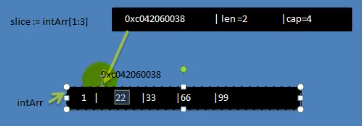
\includegraphics[width=\linewidth]{slice.png}
  \caption{切片的内部存储布局}
  \label{fig:slice}
\end{figure}

\begin{code-in-enumerate}{go}
arrays_int := [10]int{1, 2, 3, 4, 5, 6, 7, 8, 9, 10}
brrays := arrays_int
brrays[8] = 188
fmt.Printf("%v\n", arrays_int) //arrays_int的数据保持不变

slice_int := arrays_int[:]
slice_copy := arrays_int[:]

slice_int[7] = 200
fmt.Printf("%v, %v, %v\n", slice_int, slice_copy, arrays_int) //所有数据全部被修改
\end{code-in-enumerate}

  另外,和python不太一样的是,golang的切片从任何形式上来说,都是连续的。
\begin{code-in-enumerate}{go}
arrays_int := [10]int{1, 2, 3, 4, 5, 6, 7, 8, 9, 10}
slice_1 := arrays_int[3:] // 表示从数组的第3位开始往后的所有元素
slice_2 := arrays_int[:7] // 表示数组的第7位开始向前的所有元素
slice_int = arrays_int[1:3:9] // 表示从数组的前9个元素进行筛选,选取这9个元素当中的
                              // 第1到3个元素,与python的不一样!
\end{code-in-enumerate}

  Golang的map也支持切片,但是,和数组的切片不太一样,map的切片如下:
\begin{code-in-enumerate}{go}
var map_slice []map[string]string
\end{code-in-enumerate}

  \1 设计模式一:工厂模式

\begin{code-in-enumerate}{go}
// object.go
package object
type student struct {
    name string
    age  uint8
}

func (stu *student) SetName(name string) {
    stu.name = name
}

func NewStudent() *student {
    return &student{}
}

/******************/
// main.go
// package main
import object
stu := factory.NewStudent()
stu.SetName("zhangjl")
\end{code-in-enumerate}

  \1 类型断言

\begin{code-in-enumerate}{go}
usb.Start()
if p, ok := usb.(*phone); ok { // 判断usb这个接口变量是否是phone这个类型的指针,并将其赋值为p
                               // 实质上就是将接口赋值给具体类型
    p.Call()
}
usb.Stop()

switch usb.(type) { // 判断usb变量的类型
case *phone:
    fmt.Printf("It`s a phone\n")
case *camera:
    fmt.Printf("It`s a camera\n")
case *gumdan:
    fmt.Printf("It`s a gumdan\n")
}
\end{code-in-enumerate}

  \1 channel的for-range操作

  Golang当中,channel也是可以通过for-range结构进行迭代和操作的,但是,前提就是被迭代的
  channel被关闭了。如果没有被关闭,在进行for-range操作的时候,会出现死锁的问题。除此之外,
  进行for-range操作时,还有一些问题需要注意,见下方代码

\begin{code-in-enumerate}{go}
for range out_chan {
    fmt.Printf("%v\n", <-out_chan) // 无法输出out_chan当中的所有数据
                                   // 原因在于range out_chan已经从通道当中取出了一个数据
                                   // 因此,<-out_chan操作相当于取通道当中的下一个数据
}

for val := range in_chan {
    fmt.Printf("%v\n", val)       // 如果需要使用通道当中的所有结果,则必须在进行
                                  // for-range操作的时候,将通道的数据赋予另外的变量进行接收
}
\end{code-in-enumerate}

  \1 协程版本的质数求解(筛子算法)

\begin{code-in-enumerate}{go}
func generate(end int, input chan<- int) {
    for i := 2; i < end; i++ {
        input <- i
    }
    close(input)
}

func filter(input <-chan int, output chan<- int, prime int) {
    for val := range input {
        if val%prime != 0 {
            output <- val
        }
    }
    close(output)
}

func Prime(end int) chan int {
    input := make(chan int)
    output := make(chan int, end)
    go generate(end, input)
for_loop:
    for {
        prime, ok := <-input // 注意,不能使用for prime:= input的方式,原因在于input
                             // 这个通道在循环当中会不断变化
        if !ok {
            close(output)
            break for_loop
        }
        output <- prime
        tmp := make(chan int)
        go filter(input, tmp, prime)
        input = tmp
    }
    return output
}
\end{code-in-enumerate}

  \1 反射的基本要点

\begin{code-in-enumerate}{go}

// 针对普通的数据类型,其操作基本如下
func ChangeValue(in interface{}, val_in interface{}) {
    real_val := reflect.ValueOf(in).Elem()
    switch in.(type) {
    case *int:
        val := val_in.(int)
        real_val.SetInt(int64(val))
    case *int32:
        val := val_in.(int32)
        real_val.SetInt(int64(val))
    case *int64:
        val := val_in.(int64)
        real_val.SetInt(val)
    case *string:
        val := val_in.(string)
        real_val.SetString(val)
    case *float32:
        val := val_in.(float32)
        real_val.SetFloat(float64(val))
    case *float64:
        val := val_in.(float64)
        real_val.SetFloat(val)
    }
}

// 针对结构体,其操作基本如下。但是特别说明的是,针对结构体,最好是通过指针进行
// 操作,防止出现修改了之后不生效的问题出现

func ChangeStruct(struct_ptr interface{}) {
    type_pointer := reflect.TypeOf(struct_ptr)
    val_pointer := reflect.ValueOf(struct_ptr)
    val_struct := val_pointer.Elem()

    // 判断传入的参数为结构体类型的指针
    if reflect.Ptr != type_pointer.Kind() || reflect.Struct != val_struct.Kind() {
        fmt.Printf("Need struct pointer as input\n")
        return
    }

    type_struct := type_pointer.Elem()
    field_num := val_struct.NumField()
    fmt.Printf("The struct field is %d\n", field_num)
    for i := 0; i < field_num; i++ {
        fmt.Printf("The %d field name is %s , and value is %v\n", i,
            // 获取结构体字段名称,结构体对应字段的值
            type_struct.Field(i).Name, val_struct.Field(i))
        // 获取结构体包含的元素的tag标签
        tag := type_struct.Field(i).Tag.Get("json")
        if "" != tag {
            fmt.Printf("The tag of field is %v\n", tag)
        }
    }

    // 判断结构体的数据域是否可以被访问
    if val_struct.Field(1).CanSet() {
        val_struct.Field(1).SetInt(108)
        val_struct.FieldByName("Age").SetInt(120)
    }

    method_num := val_pointer.NumMethod()
    fmt.Printf("The number of struct methods is %d\n", method_num)
    for i := 0; i < method_num; i++ {
        fmt.Printf("The method name is %s, %v\n",
            // 获取结构体的方法名
            // val_pointer.Type()的结果实际上就是type_pointer
            val_pointer.Type().Method(i).Name,
            type_pointer.Method(i).Type)
    }

    // 判断结构体所包含的方法是否可以被调用
    if val_pointer.Method(0).CanAddr() {
        fmt.Printf("%v\n", val_pointer.Method(0).Call(nil)[0])
    }
}
\end{code-in-enumerate}

  \1 使用反射构造新的结构体实例

\begin{code-in-enumerate}{go}
func CreatInstance(struct_ptr interface{}) interface{} {
    struct_type := reflect.TypeOf(struct_ptr)
    strcut_struct := struct_type.Elem()
    elem := reflect.New(strcut_struct)
    instance := elem.Elem()
    instance.FieldByName("Name").SetString("zhangjl")
    instance.FieldByName("Age").SetInt(108)
    // 反射的方式调用结构体所持有的方法,调用时,所有的参数必须转换为
    // reflect.Value的切片
    params := []reflect.Value{}
    params = append(params, reflect.ValueOf(120))
    elem.MethodByName("SetAge").Call(params)
    return instance.Interface() // 必须将reflect.Value转换为interface
}

// 在main方法当中使用
obj_ := CreatInstance(obj)
if ins, ok := obj_.(factory.Obj); ok {
    fmt.Printf("%T, %s, %d\n", ins, ins.Name, ins.Age)
}
\end{code-in-enumerate}

  \1 select的基本使用与timer的重设

\begin{code-in-enumerate}{go}
// 使用过期时间的机制
intchan := make(chan struct{})
timer := time.NewTimer(3 * time.Second)
quit := make(chan struct{})
go func() {
    for i := 0; i < 10; i++ {
    add(i, i, intchan)
    }
    quit <- struct{}{}
}()

for {
    select {
    case <-intchan:
    case <-timer.C:
        fmt.Printf("Timeout for waiting\n")
        return
    case <-quit:
        fmt.Printf("quit, and reset the timer\n")
        timer.Reset(3 * time.Second) // 对timer进行重设
    }
}

// 在for-select结构当中,对退出通道进行修改
intchan := make(chan struct{})
timer := time.NewTimer(3 * time.Second)
quit := make(chan struct{}, 1) //必须用缓冲式的channel,否则会产生死锁问题
go func() {
    for i := 0; i < 10; i++ {
        add(i, i, intchan)
    }
    close(intchan)
}()

for {
    select {
    case <-intchan:
    case <-timer.C:
        fmt.Printf("Timeout for waiting\n")
        quit <- struct{}{}
        close(quit)
    case <-quit:
        fmt.Printf("quit, and reset the timer\n")
        return
    }
}
\end{code-in-enumerate}


  \1 for-select的使用误区

  For-Select是Golang并发编程当中常用的一种结构,通常与定时器ticker结合,来实现部分功能的跳转和修改。
  但是,如果使用不当,则会导致严重的CPU和内存泄漏。
\begin{code-in-enumerate}{go}
ticker := time.NewTicker(time.Second * 10)
for {
    select {
    case <-ticker.C:
        fmt.Printf("xxxxxx\n")
    default:
    }
}
\end{code-in-enumerate}

注意,上述代码是有问题的代码,由于select结构处于for循环当中,因此,只要ticker没有返回结果,
for循环就会执行select结构当中的default分支,这样的后果就是default分支占用了99\%以上的CPU时间,使得
cpu的使用率居高不下。因此,在for-select结构当中,尤其是使用定时器作为select的一个判断条件时,千万
不能随意添加default分支。上述代码应该修改为如下的形式,修改之后,大量的cpu时间则被释放,不会出现
CPU占用居高不下的情况。

\begin{code-in-enumerate}{go}
ticker := time.NewTicker(time.Second * 10)
for {
    select {
    case <-ticker.C:
        fmt.Printf("xxxxxx\n")
    }
}
\end{code-in-enumerate}


\end{outline}

\section{TimeFormat}
Go的时间格式化是比较蛋疼的,一般使用标准的格式化字符串是会有其他的字符出现的,
比如时区之类的。如果想格式化为YYYY-mm-dd HH:MM:SS或者中文时间格式,则需要使用
另外的方式。额外提示,一般的语言,包括c/c++,java以及python等等,默认的初始时间
是从1970年开始计算的,但是golang的初始时间点是2006-01-02 15:04:05.000000000 -0700 MST
\begin{code-block}{go}
const ENS_TIME_LAYOR = "2006-01-02 15:04:05"
const CHS_TIME_LAYOR = "2006年01月02日 15:04:05"
fmt.Println(time.Now().Format(ENS_TIME_LAYOR))
fmt.Println(time.Now().Format(CHS_TIME_LAYOR))
// 输出结果如下:
// 2017-08-03 15:18:15
// 2017年08月03日 15:18:16
\end{code-block}

\section{自动构建版本信息}
\begin{code-block}{go}
package main
import (
    "fmt"
)
var version = "No Version Provided"
var buildstamp = "No build stamp Provided"
var githash = "No githash Provided"
func main() {
    fmt.Printf("OceanClient Version: %s\n", version)
    fmt.Printf("OceanClient buildstamp: %s\n", buildstamp)
    fmt.Printf("OceanClient githash: %s\n", githash)
}
\end{code-block}

通过以上的代码,构建出来的版本信息是空,但是,我们可以利用go自带的一些信息,来
构建版本信息。
\begin{code-block}{bash}
go install -ldflags "-X main.version=0.1 -X \
    main.buildstamp=`date '+%Y-%m-%dT%H:%M:%S'` -X main.githash=`git rev-parse HEAD`"
\end{code-block}
其中,main表示golang的模块或者package,version、buildstamp和githash都表示package
当中的全局变量。例如:-X oceanstack/common.Version=0.1,最终的结果如下:
\begin{code-block}{bash}
/opt/github.com/learningo/bin/oceanclient version
OceanClient Version: 0.1
OceanClient buildstamp: 2018-04-25T15:37:38
OceanClient githash: 7a552b1cf6aca0e775d7b5d2dd69449cab8e783a
\end{code-block}

\section{Cobra}
Cobra是一个优秀的golang命令行参数库,提供了杰出的命令行参数处理。目前在各大商业级
的golang应用当中广泛使用。
\begin{code-block}{go}
var protocal string
var address net.IP
var port int

var conn_protocal string
var conn_address net.IP
var conn_port int

var rootcmd = &cobra.Command{
    Short: "Demo for network develop",
    Long:  ` The commands aims to show the network development`,
}

var serve = &cobra.Command{
    Use:   "serve",
    Short: "Start the network server",
    Long:  "This is the server side of the network server",
    Run:   listen,
    Args:  cobra.NoArgs, //命令行之后,除了flag之外,不接受任何参数
}

var conn = &cobra.Command{
    Use:   "connect",
    Short: "Connect the service started by serve commands",
    Long:  "This is the client side to connect the network server",
    Run:   connect,
    Args:  cobra.NoArgs,
}

func init() {

    // 追加子命令
    rootcmd.AddCommand(serve)

    // 只在子命令当中生效的flag
    serve.Flags().StringVarP(&protocal, "protocal", "p",
        "tcp", "The listen ip protocal")
    // 使用ip地址作为输入
    serve.Flags().IPVarP(&address, "ip", "i",
        net.IPv4(0, 0, 0, 0), "The listen ip address")
    serve.Flags().IntVarP(&port, "port", "n",
        8080, "The listen port")

    rootcmd.AddCommand(conn)
    conn.Flags().StringVarP(&conn_protocal, "protocal", "p",
        "tcp", "The protocal connected to ")
    conn.Flags().IPVarP(&conn_address, "ip", "i",
        net.IPv4(127, 0, 0, 1), "The connected ip address")
    conn.Flags().IntVarP(&conn_port, "port", "n",
        8080, "The port listened by server, and client connected to")
}

func listen(cmd *cobra.Command, args []string) {
    networks.Listen(protocal, address.String(), port)
}

func connect(cmd *cobra.Command, args []string) {
    networks.Connect(conn_protocal, conn_address.String(), conn_port)
}

func main() {
    // 运行cobra命令行
    if err := rootcmd.Execute(); nil != err {
        os.Exit(-1)
    }
}
\end{code-block}

\section{Golang网络编程}
\begin{outline}[enumerate]

  \1 普通的tcp/ip服务器

\begin{code-in-enumerate}{go}
func Listen(protocal, ip string, port int) {
    listener, err := net.Listen(protocal, fmt.Sprintf("%s:%d", ip, port))
    if nil != err {
        fmt.Printf("Cannot listen on port %s:%d: %v", ip, port, err)
        return
    }
    defer listener.Close()

    for {
        conn, err := listener.Accept()
        if nil != err {
            fmt.Printf("Cannot create connection :%v\n", err)
            continue
        }
        go readhandler(conn)
    }
}

func readhandler(conn net.Conn) {
    defer conn.Close()
    fmt.Printf("Connection from %s connected\n",
    conn.RemoteAddr().String())
    conn.Write([]byte("Nice to meet you !\n"))

    tmp := make([]byte, 1024)
    for {
        n, err := conn.Read(tmp)
        if io.EOF == err {
            fmt.Printf("Connection closed by remote: %s\n",
            conn.RemoteAddr().String())
            return
        }
        if nil != err {
            fmt.Printf("Failed to read from socket connection:%v", err)
            return
        }
        fmt.Printf("Recevied message from client %s:  %s\n",
        conn.RemoteAddr().String(), string(tmp[:n]))
    }
}
\end{code-in-enumerate}

  \1 普通的tcp/ip客户端

\begin{code-in-enumerate}{go}
func Connect(protocal, ip string, port int) {
    conn, err := net.Dial(protocal, fmt.Sprintf("%s:%d", ip, port))
    if nil != err {
        fmt.Printf("Cannot connect to the server %s:%d because: %v",
        ip, port, err)
        return
    }
    defer conn.Close()

    fmt.Printf("Connected the server %s:%d\n", ip, port)
    tmp := make([]byte, 1024)
    conn.Read(tmp)
    fmt.Printf("Recevied message from server :%s\n", string(tmp))

    reader := bufio.NewReader(os.Stdin)
    for {
        content, err := reader.ReadString('\n')
        if nil != err {
            fmt.Printf("Read err: %v", err)
            return
        }
        content = strings.Trim(content, " \r\n")
        if "exit" == content || "quit" == content {
            return
        }
        conn.Write([]byte(content))
    }
}
\end{code-in-enumerate}

  \1 Redis连接池
\begin{code-in-enumerate}{go}
import (
    "github.com/gomodule/redigo/redis"
)
var once sync.Once
var redispool *redis.Pool

func init() {
    once.Do(func() {
        redispool = &redis.Pool{
            MaxIdle:         3,                 // 连接池的最大空闲连接数
            MaxActive:       1024,              // 与redis的最大连接数
            IdleTimeout:     120 * time.Second, // 连接的最大空闲时间
            MaxConnLifetime: 10 * time.Minute,

            Dial: func() (redis.Conn, error) {
                return redis.Dial("tcp", "10.1.4.24:6379")
            },
            TestOnBorrow: func(c redis.Conn, t time.Time) error {
                if time.Since(t) < time.Minute {
                    return nil
                }
                _, err := c.Do("PING")
                return err
            },
        }
    })
}
\end{code-in-enumerate}

  \1 Grpc实现服务器到客户端的通信

  通常来说,服务器客户端之间的交互属于一个请求应答模式,即客户端发起请求,服务器进行对应的回复。
  如果需要由服务器端单独向客户端发送消息,在常见的Rest模式下基本不太可能,毕竟Rest属于短连接。
  一般的情况,如果做这种交互操作,需要使用TCP的方式,或者借助消息队列的模式。不过,可以通过对
  Grpc的部分修改,达到这个目的。下面的例子当中,我们通过一个模拟来实现这个功能:客户端启动之后,
  向服务器发送一个订阅的请求,服务器根据这个订阅的请求,定时的向客户端发送消息。而这个定时的发送
  功能,可以根据需要,在服务端接收到其他请求之后,再进行发送。
\begin{code-in-enumerate}{go}
// protoc 描述文件
syntax = "proto3";
package messages;
service RegisterSrv{
    rpc Subscribe (stream Topic) returns (stream Notification) {} // 需要使用stream流模式,进行双工通信
}

message Topic {
    string client = 1;
}

message Notification {
    string client = 1;
    string server = 2;
    string msg = 3;
}
\end{code-in-enumerate}

  服务器端的代码如下:
\begin{code-in-enumerate}{go}
type Streamer struct {
    name      string
    substream map[string]messages.RegisterSrv_SubscribeServer
}

func NewStreamer() *Streamer {
    return &Streamer{
        name:      "PushNotifyServer",
        substream: make(map[string]messages.RegisterSrv_SubscribeServer),
    }
}

func (this *Streamer) Subscribe(stream messages.RegisterSrv_SubscribeServer) error {
    var client string = ""
    for {
        input, err := stream.Recv()
        if io.EOF == err {
            fmt.Printf("Complete recv\n")
            if "" != client {
                delete(this.substream, client)
            }
            return nil
        }
        if nil != err {
            fmt.Printf("Error: %v\n", err)
            if "" != client {
                delete(this.substream, client)
            }
            return err
        }
        client = input.GetClient()
        fmt.Printf("Received a Subscription Request (%s, %s)\n",
            client, input.String())
        _, ok := this.substream[client]
        if !ok {
            this.substream[client] = stream
        } else {
            fmt.Printf("Client %s already subscribed\n", client)
        }
    }
    return nil
}

func (this *Streamer) pushmsg() {
    ticker := time.NewTicker(10 * time.Second)
    for {
        select {
        case <-ticker.C:
            for client, server := range this.substream {
                fmt.Printf("Server send message to client:%s\n", client)
                    server.Send(&messages.Notification{
                        Client: client, Server: "push server",
                        Msg: fmt.Sprintf("From server to client %s: %s",
                    client, time.Now().Format("2006-01-02 15:04:05.000000000"))})
            }
        }
    }
}

func main() {
    grpc_server := grpc.NewServer()
    service := NewStreamer()
    messages.RegisterRegisterSrvServer(grpc_server, service)
    address, err := net.Listen("tcp", "0.0.0.0:8080")
    if nil != err {
        panic(err)
    }

    go service.pushmsg()
    defer address.Close()
    reflection.Register(grpc_server)
    if err = grpc_server.Serve(address); nil != err {
        panic(err)
    }
}
\end{code-in-enumerate}

  客户端的代码如下:
\begin{code-in-enumerate}{go}
func subscribe(client messages.RegisterSrvClient, name string) {
    stream, err := client.Subscribe(context.Background())
    if nil != err {
        fmt.Printf("Failed to subscribe the channel:%v\n", err)
        return
    }

    if err := stream.Send(&messages.Topic{Client: name}); nil != err {
        fmt.Printf("Cannot send message to subscribe server:%v\n", err)
        return
    }
    notification(stream)
}

func notification(stream messages.RegisterSrv_SubscribeClient) {
    for {
        resp, err := stream.Recv()
        if io.EOF == err {
            stream.CloseSend()
            return
        }
        if nil != err {
            fmt.Printf("Cannot recevied anything:%v\n", err)
            stream.CloseSend()
            return
        }
        fmt.Printf("Recevied message: %s\n", resp.GetMsg())
    }
}

func main() {
    conn, err := grpc.Dial("172.16.11.151:8080", grpc.WithInsecure())
    if nil != err {
        fmt.Printf("Failed to connect the grpc server :%v\n", err)
        return
    }
    defer conn.Close()
    client := messages.NewRegisterSrvClient(conn)

    rand.Seed(time.Now().UTC().UnixNano())
    name := fmt.Sprintf("%s:%d", "Client", rand.Intn(50))
    subscribe(client, name)
}
\end{code-in-enumerate}

  整体的运行结果如下图所示\nameref{fig:grpc}。
\begin{figure}[H]
  \centering
  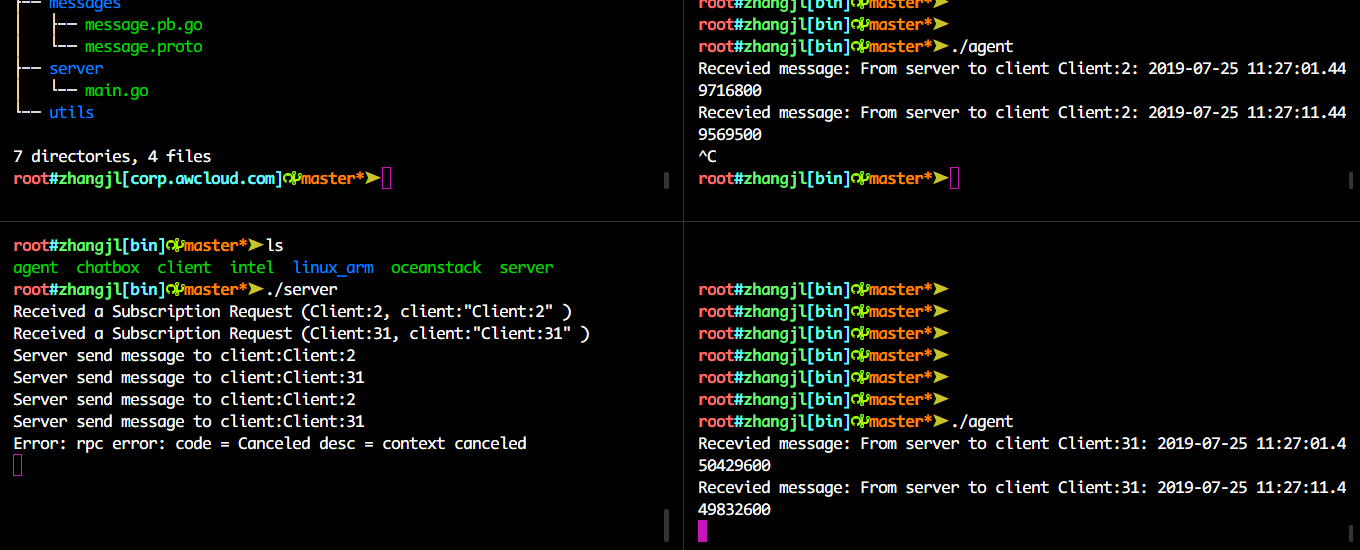
\includegraphics[scale=0.2]{grpc.png}
  \caption{Grpc服务端客户端双工通信}
  \label{fig:grpc}
\end{figure}

\end{outline}
